
\subsection{Characteristics of the network}

The network we used consists of 384 nodes. The distribution of the number of friends and the local clustering coefficients are shown in Figure \ref{hist1}. The one of the betweenness centrality in Figure \ref{hist2}.


\begin{minipage}{0.5\textwidth}
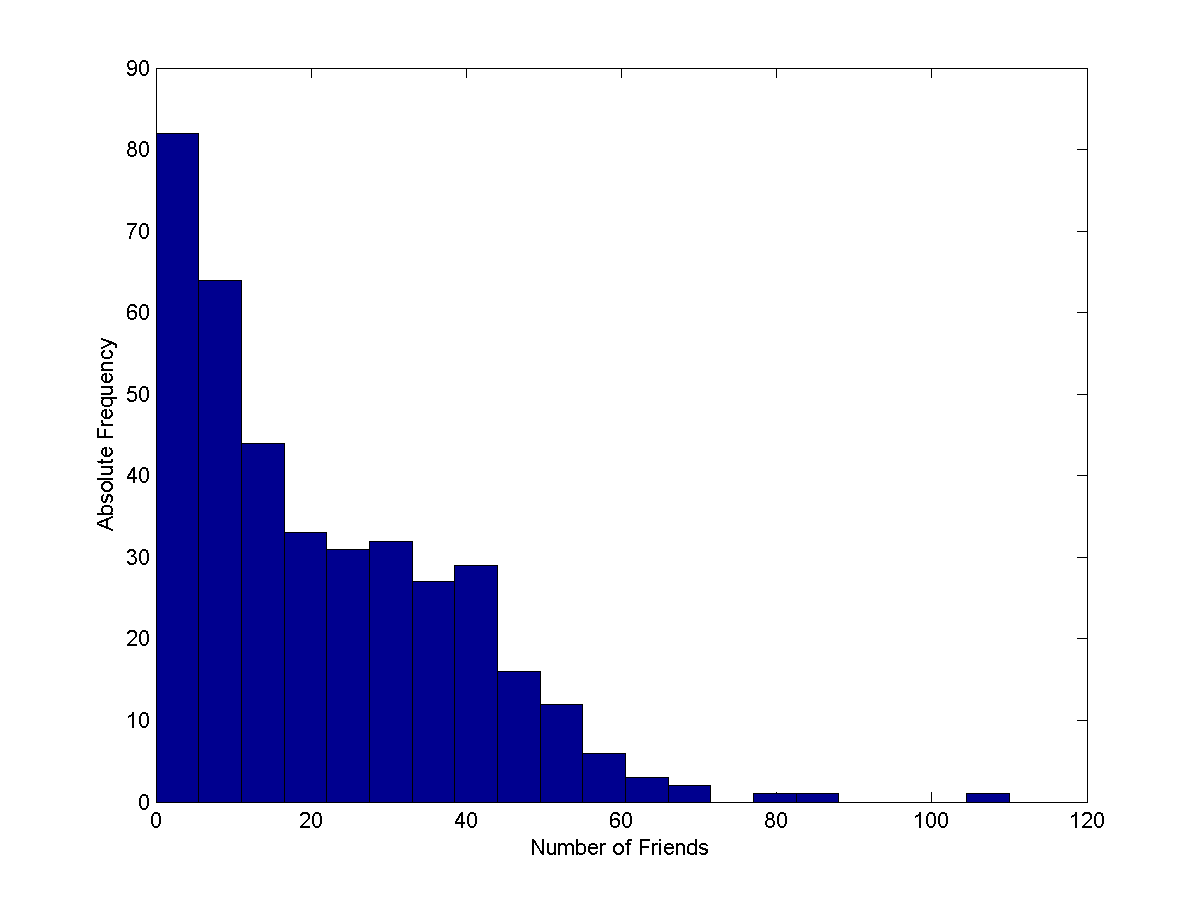
\includegraphics[width=7cm]{network_degreehist.png}
\end{minipage}
\begin{minipage}{0.5\textwidth}
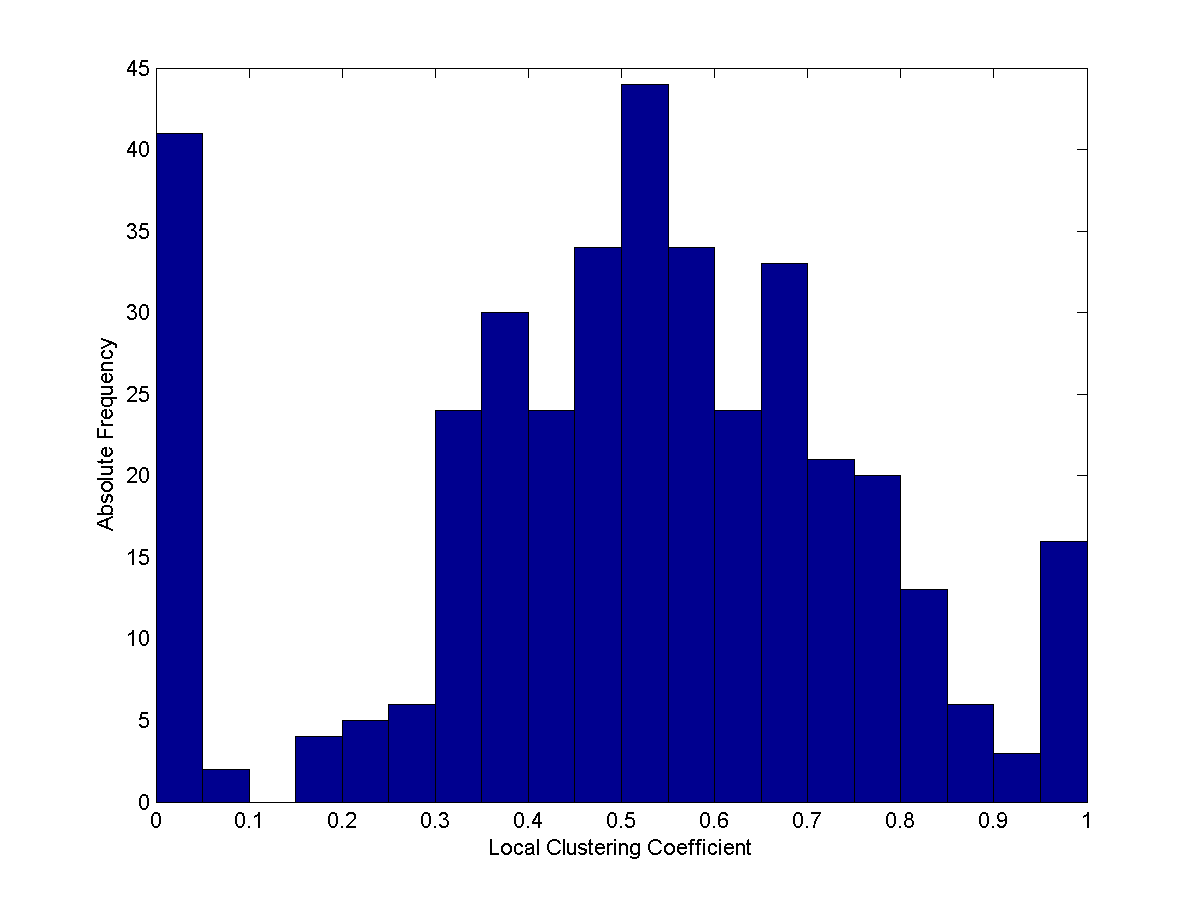
\includegraphics[width=7cm]{network_clusterhist.png}
\end{minipage}
\captionof{figure}{Distribution of the number of friends (left) and the local clustering coefficient (right).}
\label{hist1}


\begin{minipage}{0.5\textwidth}
The main problem of our network is, that it consists of all the friends of one of the authors, with the author removed. The probability of infecting another person was dependent on the mutual friends, so it's possible that two individuals have a lot of common friends in reality, but it appears that they don't because the author doesnn't know these common friends.
\end{minipage}
\begin{minipage}{0.5\textwidth}
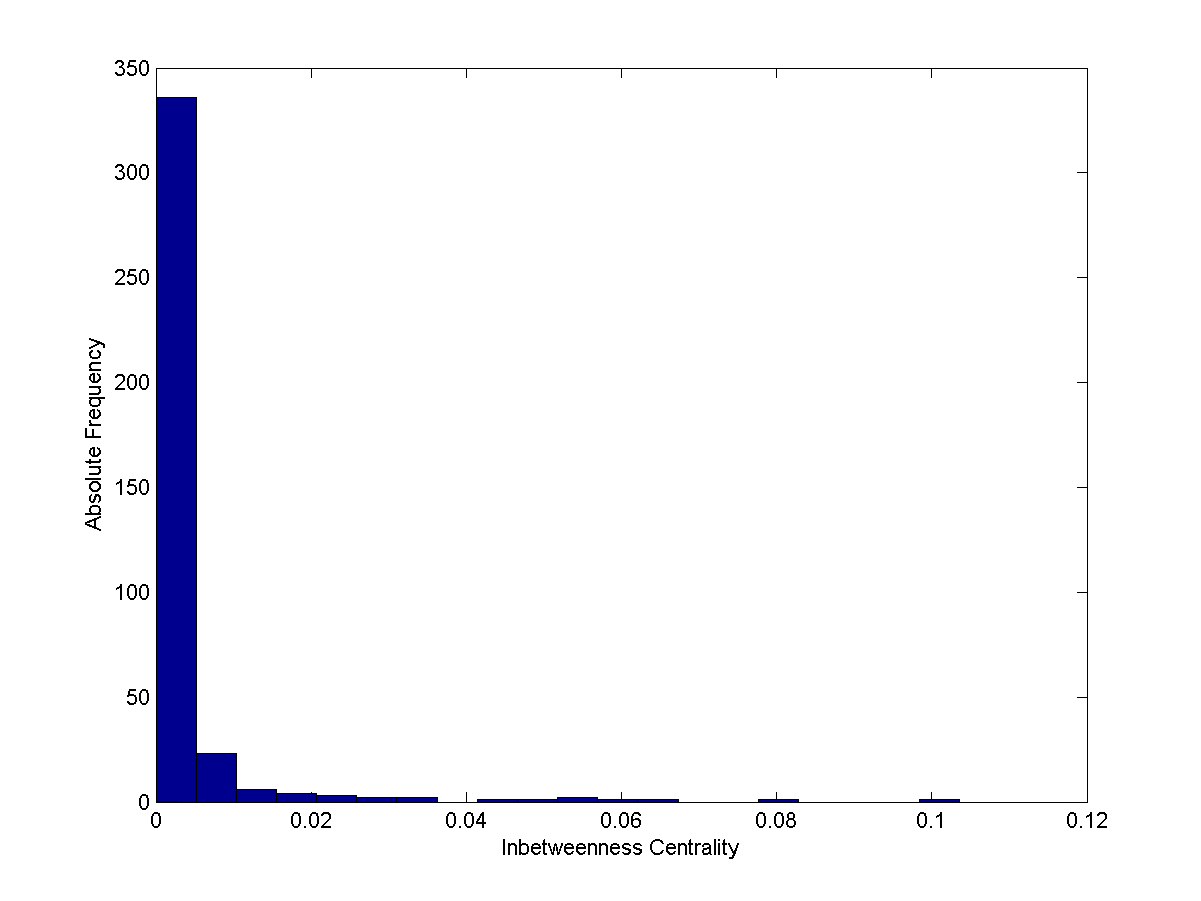
\includegraphics[width=7cm]{network_centralityhist.png}
\captionof{figure}{Distribution of betweenness centrality.}
\label{hist2}
\end{minipage}

%\begin{minipage}{0.33\textwidth}
%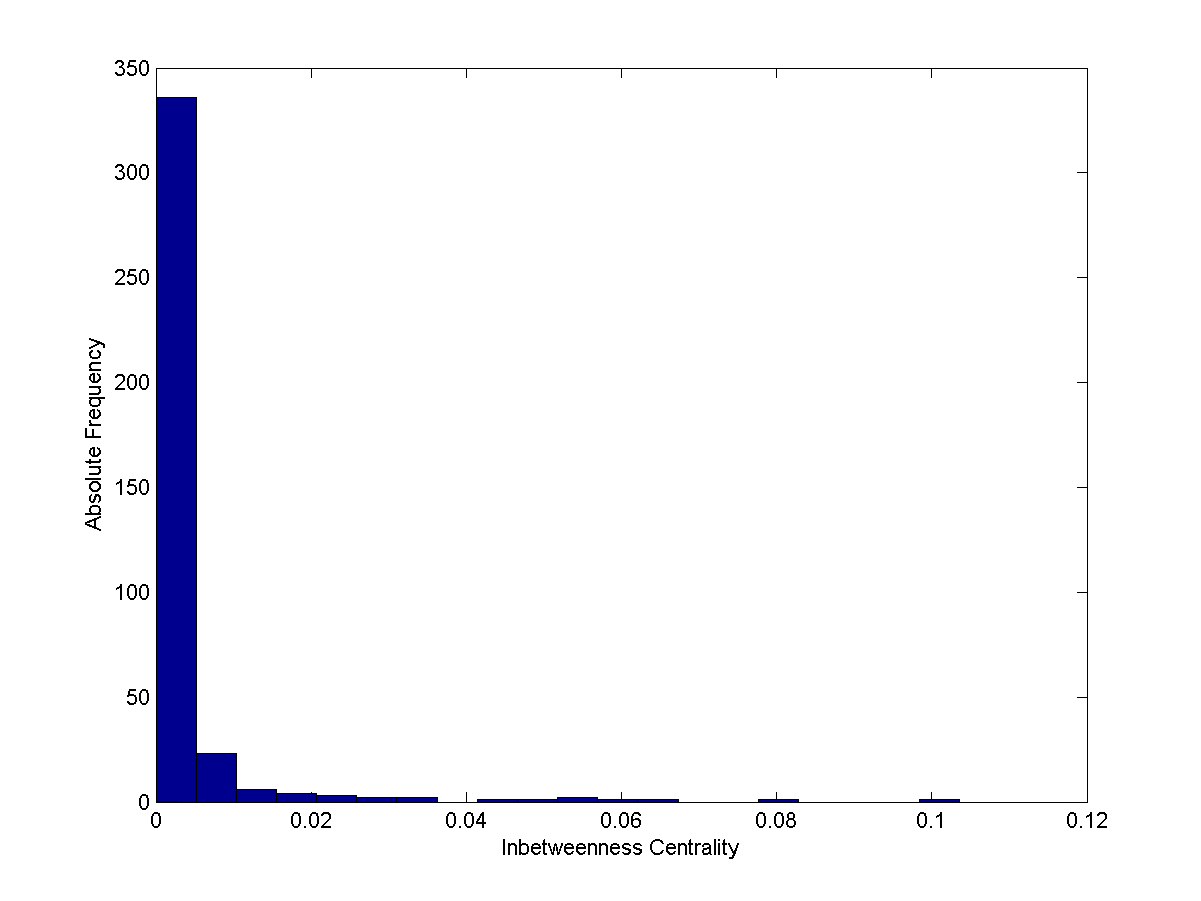
\includegraphics[scale=0.3]{network_centralityhist.png}
%\end{minipage}



\subsection{Differences in the time evolution}

Most of the time, the form of the evolution graph of the system looks very similar in the case of the homogeneous and the inhomogeneous, agent-based model (Figure \ref{evolution1}).

\begin{minipage}{0.5\textwidth}
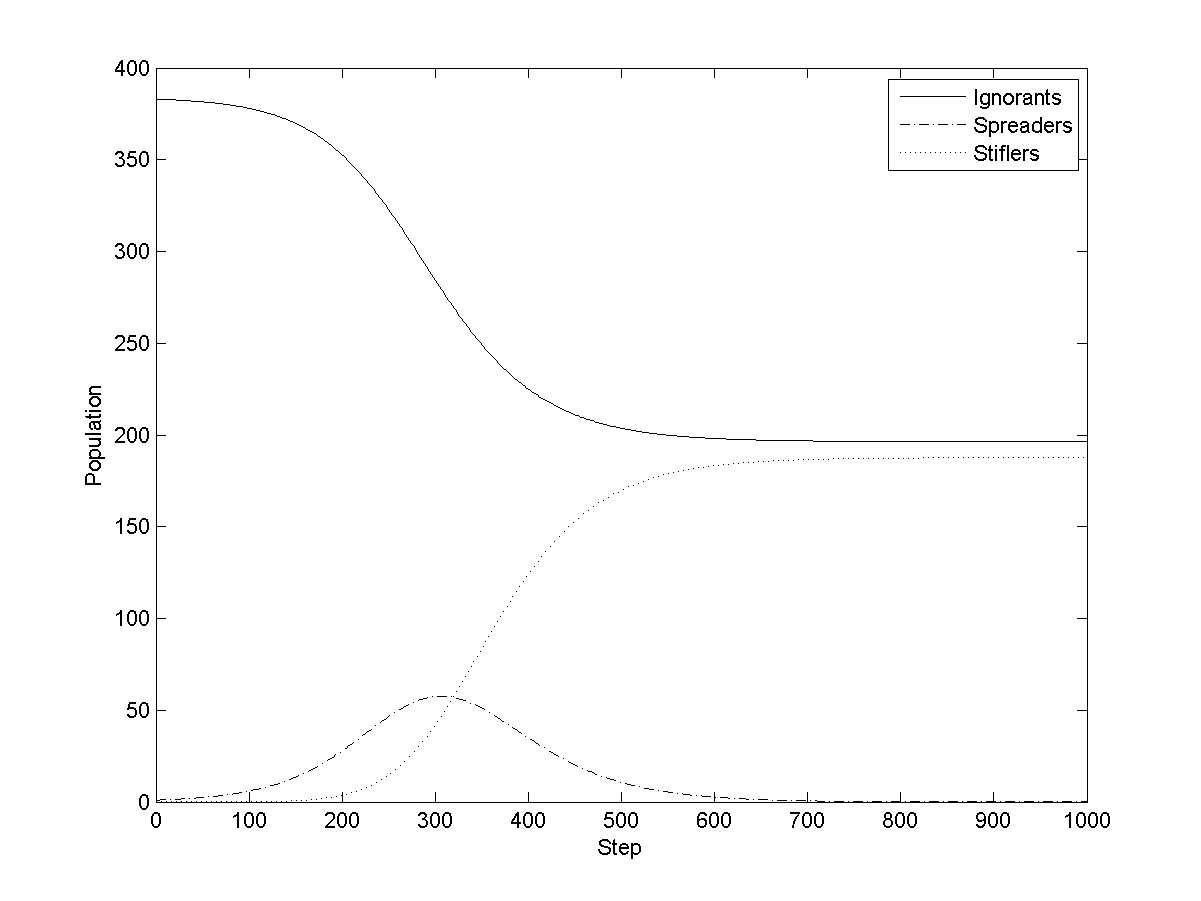
\includegraphics[width=7cm]{NICE_SIR}
\end{minipage}
\begin{minipage}{0.5\textwidth}
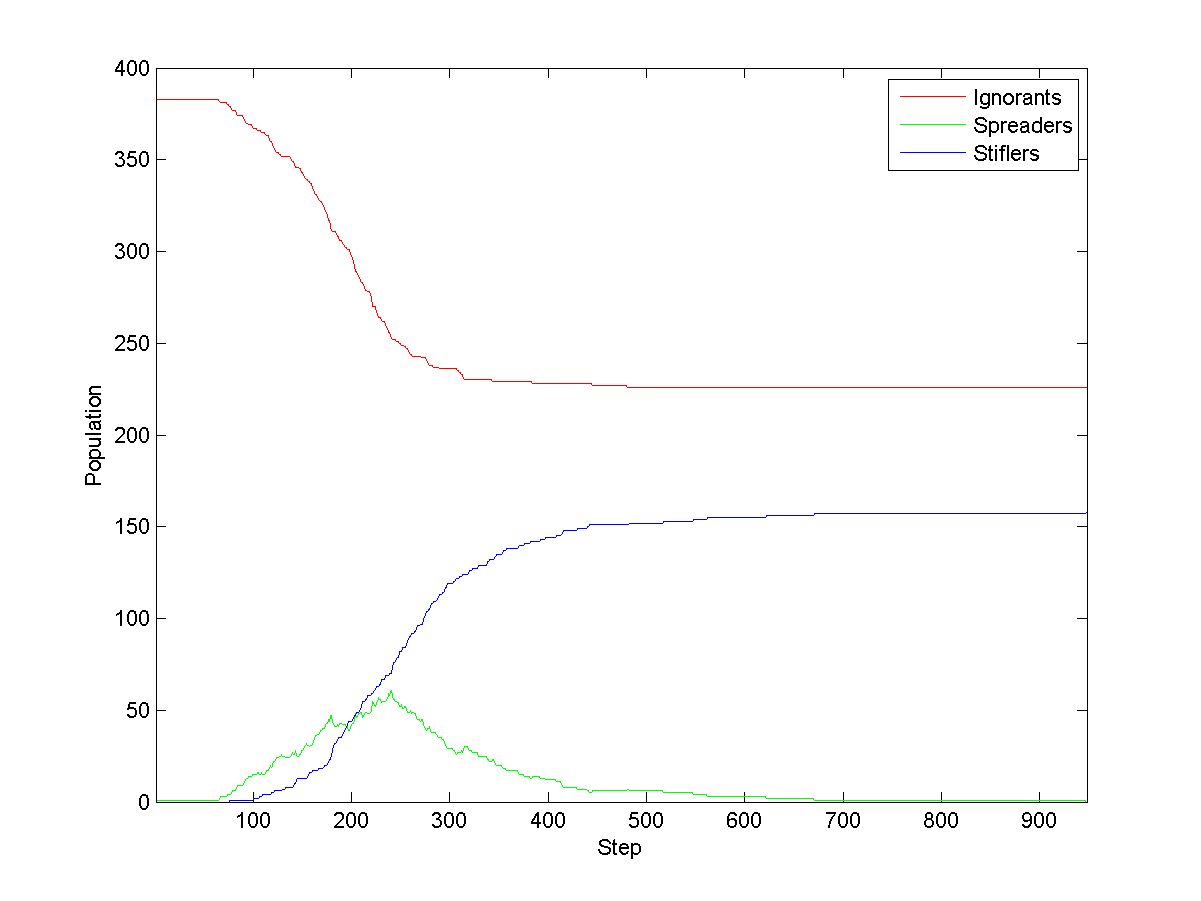
\includegraphics[width=7cm]{1-local-max}
\end{minipage}
\captionof{figure}{Left: Typical evolution of the system in the homogeneous SIR-model. Right: The Evolution in the agent-based model. In most cases, the evolution looks somewhat like this.\newline}
\label{evolution1}


\begin{minipage}{0.5\textwidth}
But there were also interesting cases where two local maxima occurred, as in Figure \ref{2peaks}. This can never be the case in a homogeneous model. This requires several neighbourhoods in the network (and some luck, since the simulation uses random numbers). This might be a rather obvious insight, but it proofs that a homogeneous model might fail totally. If you would base any decision on a homogeneous model and you recognize that the number of spreaders decreases, you would expect that the spreading comes to an end. But it might be  that it hardly started if you have inhomogeneities.
\end{minipage}
\begin{minipage}{0.5\textwidth}
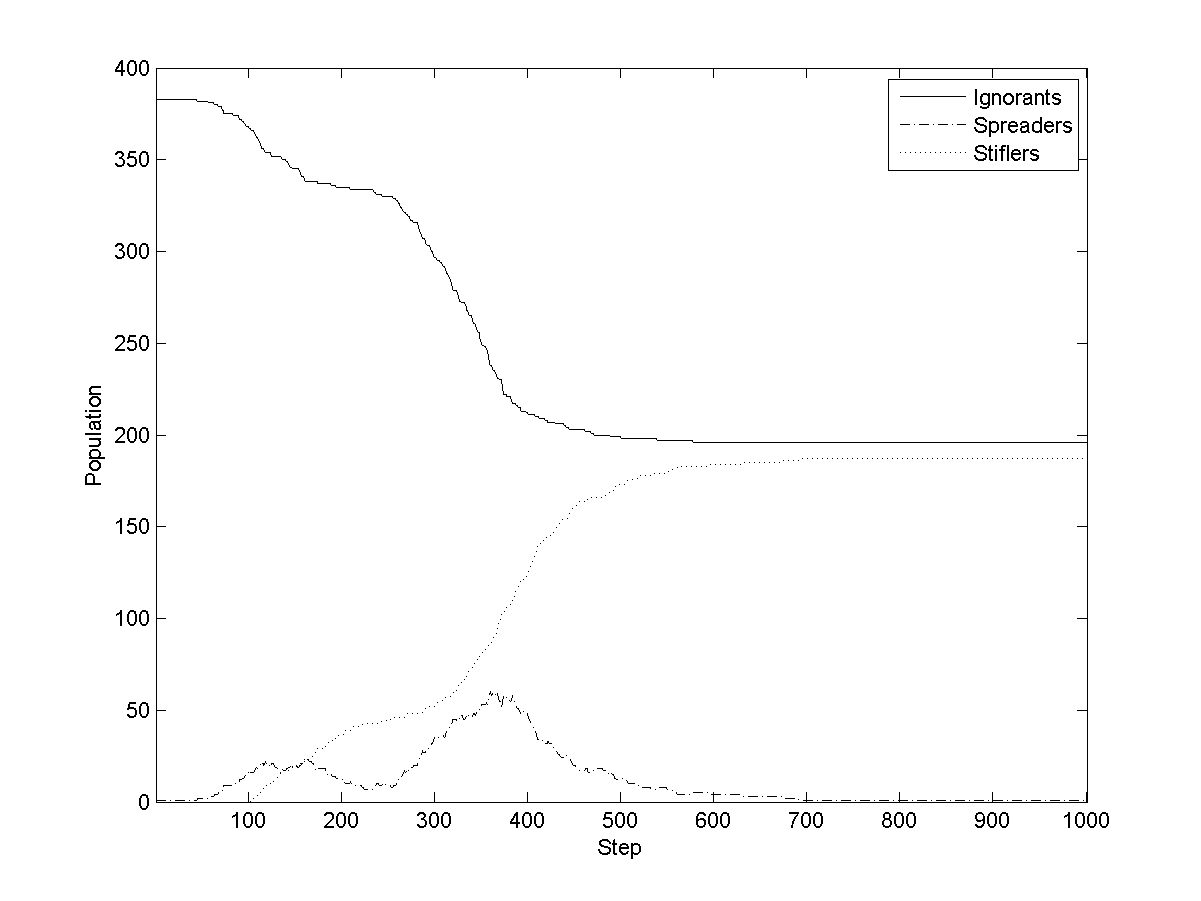
\includegraphics[width=7cm]{2-local-max}
\captionof{figure}{two local maxima, not continuous}
\label{2peaks}
\end{minipage}


\subsection{Influence of $\alpha$}


In the big simulation conducted $\alpha$ was assigned the value 0.3. This value was chosen because higher values limit the information spreading to a large number of individuals, whereas small numbers increase computing time significantly. In another simulation the influence of $\alpha$ was investigated by simulating the information spreading 25 times for 20 different values of $\alpha$ between 0.05 and 1, while starting always with the same spreader. In figure \ref{Analysis_pforget} the average number of remaining spreaders at the end of the simulation is plotted against $\alpha$. Figure \ref{Analysis_pforget_ODE} shows the number of remaining spreaders vs. $\alpha$ obtained with the homogeneous model. The resemblance of those two figures implies that both models behave similarly with respect to $\alpha$. Even though  it was not investigated, we assume that $\alpha$ does not influence the importance of individuals in the network.

\begin{minipage}{0.5\textwidth}
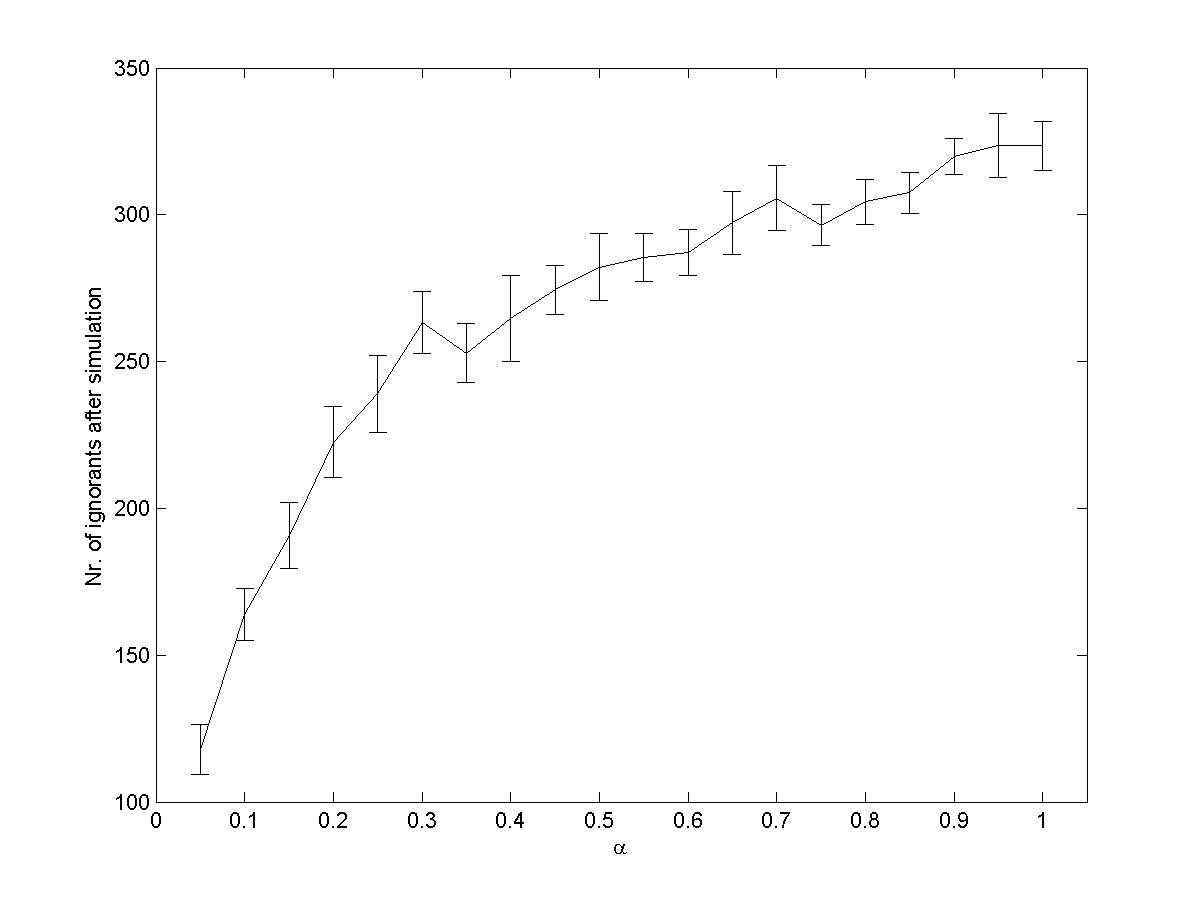
\includegraphics[width=7cm]{Analysis_pforget}
\captionof{figure}{Influence of $\alpha$ in the \newline agent-based model.}
\label{Analysis_pforget}
\end{minipage}
\begin{minipage}{0.5\textwidth}
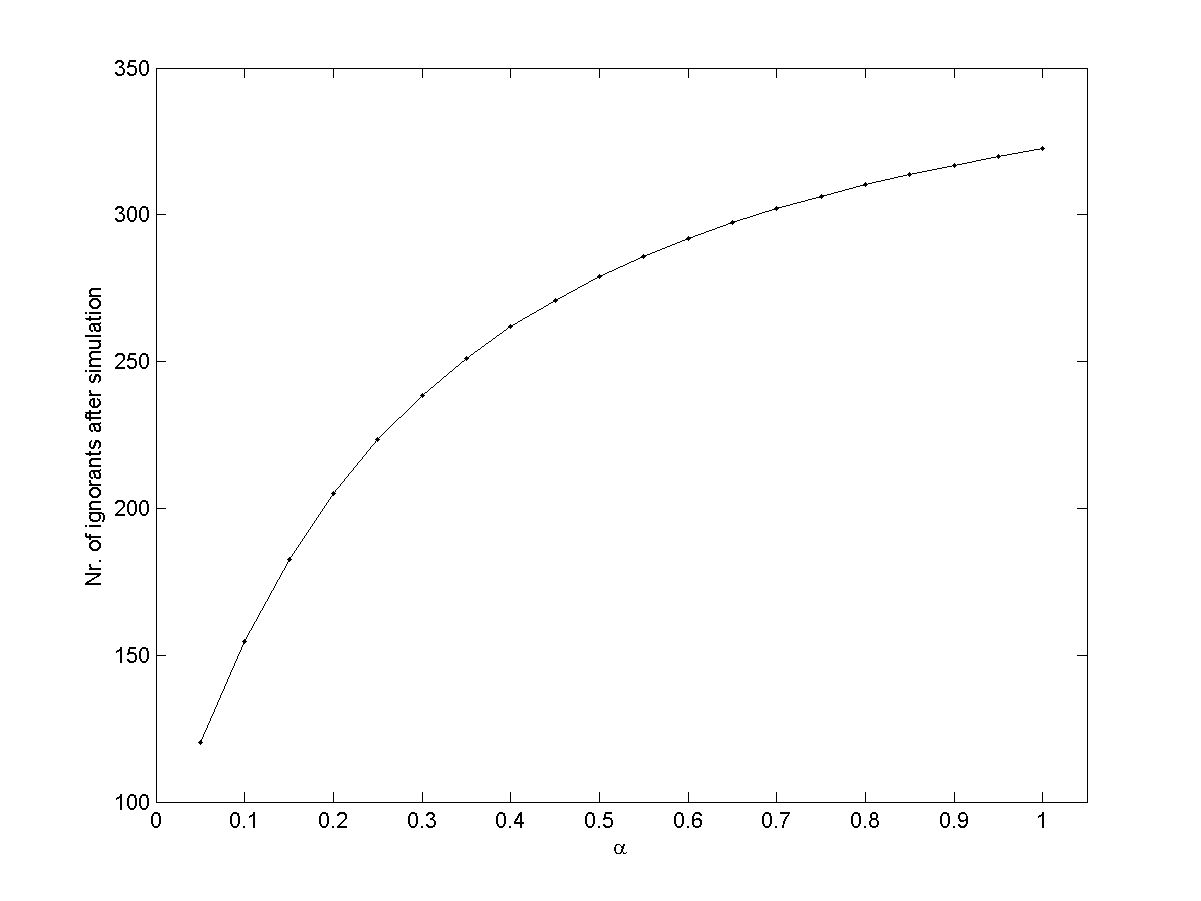
\includegraphics[width=7cm]{Analysis_pforget_ODE}
\captionof{figure}{Influence of $\alpha$ in the \newline homogeneous model.}
\label{Analysis_pforget_ODE}
\end{minipage}




\subsection{Influentials}

\subsubsection{Existance and Imprtance of Influentials}

\begin{minipage}{0.5\textwidth}
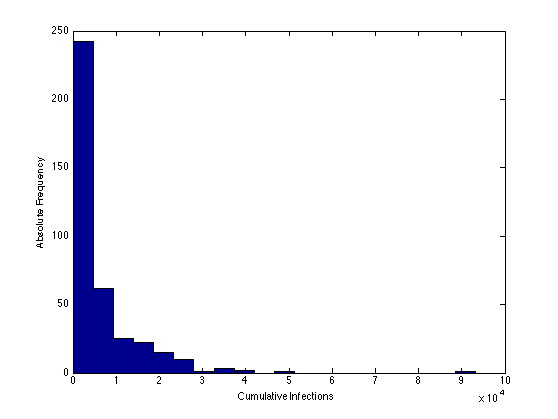
\includegraphics[width=7cm]{influ2}
\caption{Distribution of the cumulative infections, summed over all 3840 rounds. \newline}
\label{Histo}
\end{minipage}
\begin{minipage}{0.5\textwidth}
Figure \ref{Histo} is a simple histogram that shows that the vast majority of people has only a small cumulative infection value. However, there are some individuals with a very high value. This an indicator for the existence of influentials.   \\
\end{minipage}

%\begin{figure}[H!]
%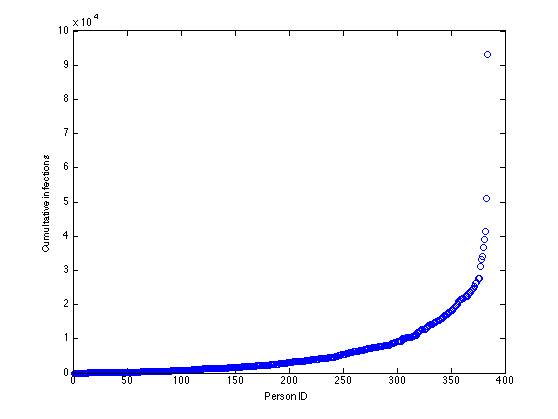
\includegraphics[width=7cm]{influ1}
%\caption{sdlhfa}
%\label{Sorted}
%\end{figure}



\noindent One can even go one step further and try to estimate the importance of those influentials on all infections that occurred in total. In order to do so, the persons are sorted according to their value of cumulative infections. Then, for each person m, we sum up all the infections that occurred in rounds where m itself did NOT infect anybody. Let's call this function f(m). Figure \ref{importancedist} shows the value of $$g(m)=\sum_{i=1}^m f(i) $$
This can be interpreted as the number of infections that occurred in rounds where all persons more or equally important than m did NOT infect anybody. So $g(1)=0$ and $g_{max}=$total infections.
\\
Given these results, we get that 94\% of all infections happen in the rounds where the 1\%-quantile of the most important people were not excluded. 


\begin{minipage}{0.5\textwidth}
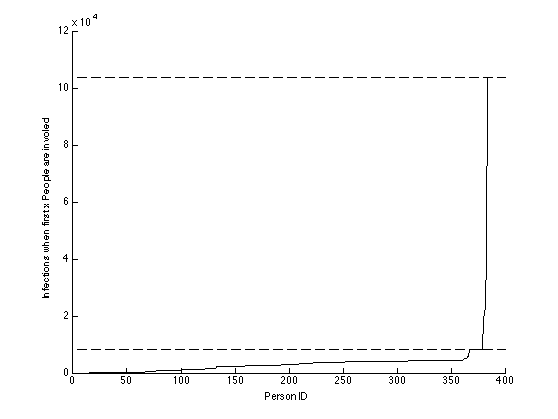
\includegraphics[width=7cm]{influ3}
\end{minipage}
\begin{minipage}{0.5\textwidth}
\caption{ g(m) (see above for details). The bottom dashed line indicated the number of all infections in rounds where the four most important individuals did not infect anybody(6\% of all infections). The top dashed line shows the total number of infections in all 3840 rounds in the simulation.}
\label{importancedist}
\end{minipage}

\noindent This result seems to proof the existence of influentials in our network. However, one could say that this only shows that the so called influentials are just contributing in rounds where many persons get infected, not that this is caused by the influentials. But they are also the ones with the most cumulative infections, which shows that they really \textit{cause} a high number of infections.


\subsubsection{Determine influentials}


The next question is, whether it is possible to determine parameters that indicate influentials. e.g. the number of friends or the cluster coefficient.
\\
We were not able to identify a single parameter which clearly predicts the influentials. We recognized that persons with a higher number of friends and a higher activity infect more people directly, they also have a higher number of cumulative infections, but the influentials or the persons with the highest number of cumulative infections are  NOT all following this trend. The best indicator we have is the betweenness centrality: The two persons with the highest number of cumulative infections are the two with the highest betweenness centrality (Figure \ref{Betweenness}). But a higher betweenness centrality does not indicate a higher importance. Persons with a higher betweenness centrality connect different neighbourhoods, so their importance may come from the fact that they are one of the few persons which are able to connect large groups of persons which would be isolated without these linkers.

 




\begin{minipage}{0.5\textwidth}
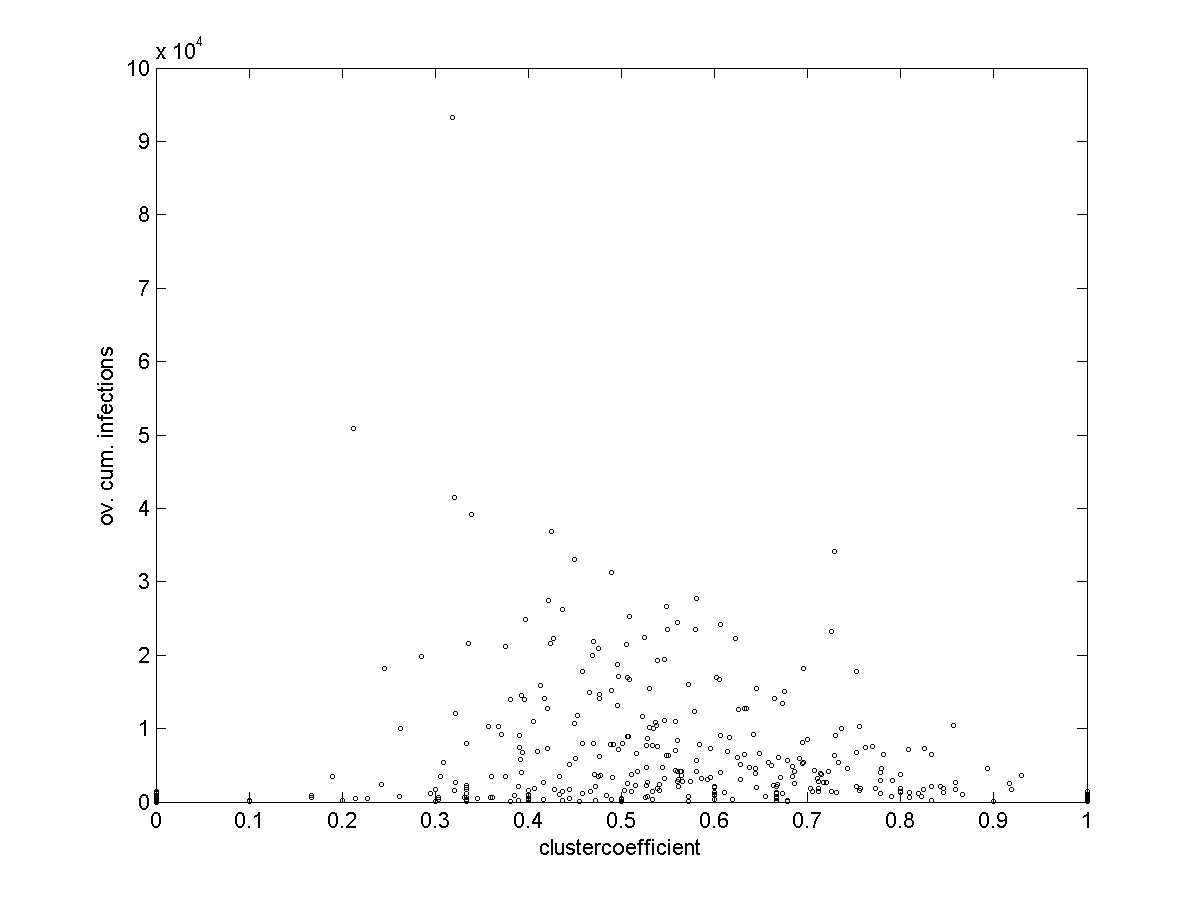
\includegraphics[width=7cm]{clustercVSov_cum_inf}
\end{minipage}
\begin{minipage}{0.5\textwidth}
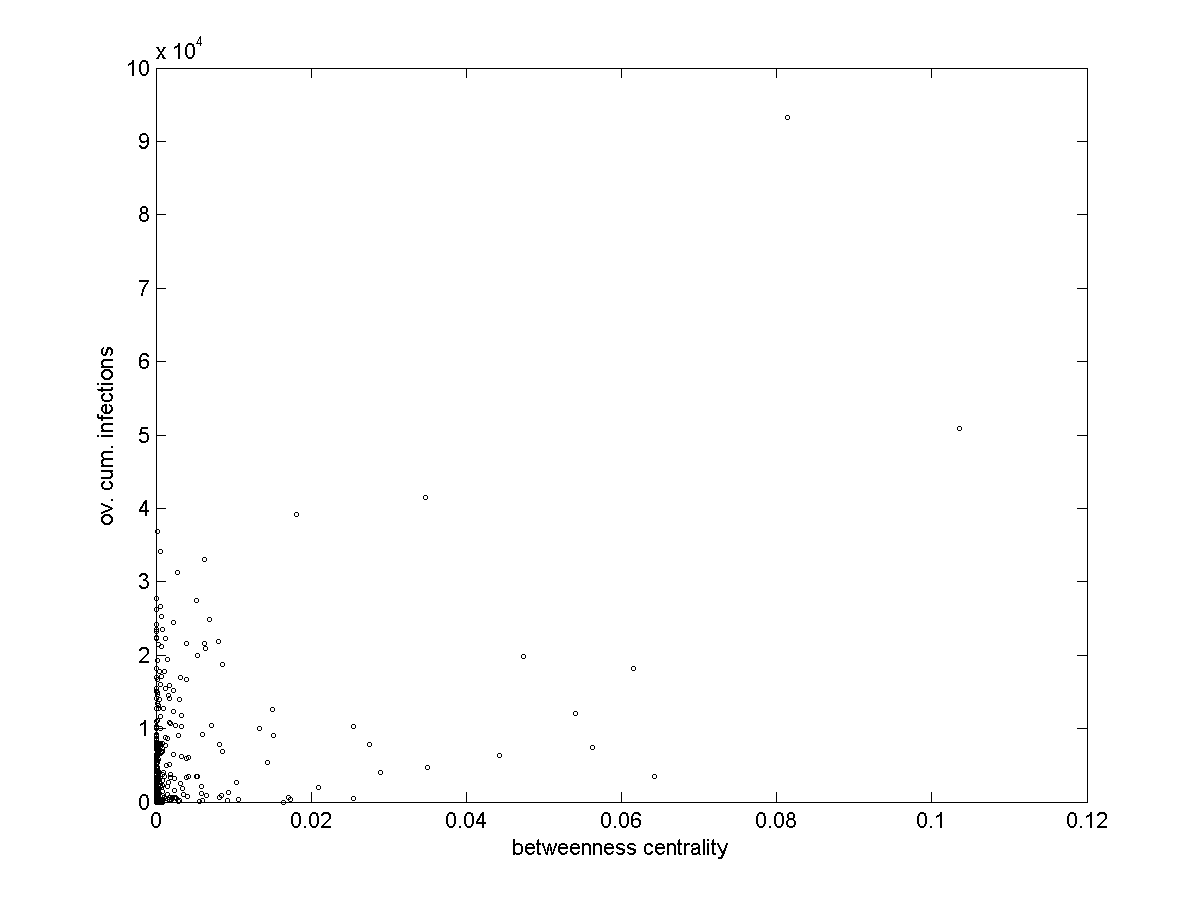
\includegraphics[width=7cm]{betwVSov_cum_inf}
\end{minipage}
\captionof{figure}{Left: Cumulative Infections in all rounds vs. the cluster coefficient. A higher cluster coefficient does obviously not indicate a higher number of cumulative infections. On the contrary, within our model, very clustered persons can become spreaders fast, but they also become stiflers fast, limiting the possibility that the "disease" reaches other neighbourhoods. Right: Cumulative infections vs. betweenness centrality. The two persons with the highest betweenness centrality also have the highest number infections.  }
\label{Betweenness}








